\scanpage{8}
\mspage{\textcircled{3}}
% archive foliation: 7
\[
\boxed{H_A(\Phi,\Psi)=\mathrm{Hom}_{\widehat A}(\Phi,\psi_A(\Psi))\simeq\mathrm{Hom}_{A^\vee}(\Psi,\varphi_A(\Phi))}
\]
\diagram{\begin{tikzcd}[row sep=tiny,column sep=small]
\Phi&\Psi\\
\mathrm{Ob}\widehat A\arrow[u]&\mathrm{Ob}A^\vee\arrow[u]
\end{tikzcd}}
\margin{\diagram{\boxed{\begin{array}{ccc}
\widehat A^\circ&\xrightarrow{\varphi_A}&A^\vee\\
A^{\vee\circ}&\xrightarrow{\psi_A}&\widehat A\\
\widehat A^\circ\times A^{\vee\circ}&\xrightarrow{H_A}&\mathrm{Ens}
\end{array}}}}

i.e. on a
\diagram{\begin{tikzcd}
A^{\vee\circ}\arrow[r,shift right=1.2ex,no head,"\psi_A"']&\widehat A\arrow[l,shift right=1.2ex,"\varphi_A^\circ"']
\end{tikzcd}}
ou
\diagram{\begin{tikzcd}
A^\vee\arrow[r,shift left=1.2ex,no head,"\psi_A^\circ"]&\widehat A^\circ\arrow[l,shift left=1.2ex,"\varphi_A"]
\end{tikzcd}}
paires de foncteurs adjoints

\uline{NB}

a) \diagram{\begin{tikzcd}[row sep=small]
A^{\vee\circ}\arrow[rr,"\psi_A"]&&\widehat A\\
&A\arrow[ul,hook,"h^A"]\arrow[ur,hook,"h_A"']&
\end{tikzcd}}
commutatif, et $\psi_A$ commute aux $\underset{\leftarrow}{\lim}$
-- ce qui caractérise $\psi_A$ à iso unique près

b) \diagram{\begin{tikzcd}[row sep=small]
A^{\vee\circ}&&\widehat A\arrow[ll,"\varphi_A^\circ"']\\
&A\arrow[ul,hook,"h^A"]\arrow[ur,hook,"h_A"']&
\end{tikzcd}}
commutatif, et $\varphi_A^\circ$ commute aux $\underset{\rightarrow}{\lim}$
et cela caractérise $\varphi_A^\circ$ à iso unique près

\margin{\figure{\begin{tikzpicture}\node[inner sep=3pt] (nb) {\begin{minipage}{.34\linewidth}\uline{NB}
$\left\{\begin{aligned}\varphi_{A^\circ}&=\psi_A\\\psi_{A^\circ}&=\varphi_A\\H_{A^\circ}&={}^sH_A\end{aligned}\right.$ i.e.
$H_{A^\circ}(\Psi,\Phi)=H_A(\Phi,\Psi)$
(fonctoriel en $\Phi,\Psi$)
\unsure{\S}\end{minipage}};\draw (nb.north west)--(nb.north east)--(nb.south east)--(nb.south west);\end{tikzpicture}}}

\[
\boxed{\Phi\xrightarrow{\alpha_\Phi}\psi_A\varphi_A^\circ(\Phi)}\quad\text{dans }\widehat A
\qquad\text{i.e.}\qquad
\Phi\longleftarrow\psi_A^\circ\varphi_A(\Phi)\quad\text{dans }\widehat A^\circ
\]
\[
\Psi\longleftarrow\varphi_A^\circ\psi_A(\Psi)\quad\text{dans }A^{\vee\circ}
\qquad\text{i.e.}\qquad
\boxed{\Psi\xrightarrow{\beta_\Psi}\varphi_A\psi_A^\circ(\Psi)\quad\text{dans }A^\vee}
\]
\unsure{\S} morphismes d'adjonction

iso si $\Phi\in\mathrm{Ob}\,A$ ou $\Psi\in\mathrm{Ob}\,A$

c) \(\boxed{H_A(a,b)=\mathrm{Hom}_A(a,b)}\)
\diagram{\begin{tikzcd}[row sep=tiny,column sep=small]
a\arrow[d]&b\arrow[d]\\
\text{pour }h_A(a)&\text{pour }h^A(b)
\end{tikzcd}}
donc $H_A$ prolonge $\mathrm{Hom}_A$, et est caractérisé à iso unique près par cette propriété,
plus celle que $H_A$ commute aux $\underset{\leftarrow}{\lim}$
\inserted{\[
\left[\begin{aligned}
H_A(\Phi,b)&\simeq\mathrm{Hom}_{\widehat A}(\Phi,b)\\
H_A(a,\Psi)&\simeq\mathrm{Hom}_{A^\vee}(\Psi,a)=\mathrm{Hom}_{A^{\vee\circ}}(a,\Psi)
\end{aligned}\right]
\]}
\figure{
\begin{tikzpicture}\draw[->,double](0,.5)--(-.3,0);\end{tikzpicture}}

\uline{Question} Que peut-on dire des morphismes d'adjonction
$\alpha_\Phi,\beta_\Psi$ ? Iso (si et) seulement si $\Phi$ resp. $\Psi$ est représentable ?

\unsure{Est-ce|Est-on} tjrs une équivalence faible (sans doute pas).

Les foncteurs $\varphi_A$ et $\psi_A$ transforment-ils équiv. faibles en isom ?

Relation aux contractions
\[
\boxed{H^A:\quad(\Phi,\Psi)\longmapsto\Phi\mathbin{\ast_A}\Psi\ ;\quad
\widehat A\times A^\vee\underset{!!}{\longrightarrow}\mathrm{Ens}}
\]
d) \(\boxed{H^A(a,b)\overset{\inserted{\text{ou}}}{=}\mathrm{Hom}_A(b,a)}\)
\diagram{\begin{tikzcd}[row sep=tiny,column sep=small]
a\arrow[d]&b\arrow[d]\\
\text{pour }h_A(a)&\text{pour }h^A(b)
\end{tikzcd}}
et $\unsure{H^A_A|H^A}$ commute aux $\underset{\rightarrow}{\lim}$, ce qui le caractérise à iso. unique près
\[
\deleted{\unsure{\varphi^A}\unsure{H_A(a)}\unsure{\ne|=}}
\qquad\boxed{\begin{aligned}\Phi\ast a&=\Phi(a)\\a\ast\Psi&=\Psi(a)\end{aligned}}
\]
\diagram{\boxed{\begin{array}{ccc}
\widehat A&\xrightarrow[\simeq]{\varphi^A}&\underline{\mathrm{Hom}}_!(A^\vee,\mathrm{Ens})\\
A^\vee&\overset{\psi^A}{\underset{\simeq}{\rule{1.2cm}{.3pt}}}&\underline{\mathrm{Hom}}_!(\widehat A,\mathrm{Ens})
\end{array}}}
\figure{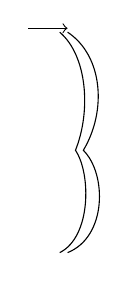
\begin{tikzpicture}\draw(0,0)..controls(.4,.2)and(.4,1)..(.2,1.3)..controls(.4,1.8)and(.35,2.5)..(0,2.8);\draw(.1,0)..controls(.6,.2)and(.6,1)..(.3,1.3)..controls(.6,1.8)and(.55,2.5)..(.1,2.8);\draw[->](-.4,2.85)--(.1,2.85);\end{tikzpicture}}
\unsure{\S}
\[
\boxed{H^A(\Phi,\Psi)=\deleted{\unsure{\Phi}}\varphi^A(\Phi)(\Psi)\simeq\psi^A(\Psi)(\Phi)}
\]

\texttt{/*}\unsure{\texttt{JOBPARM}}\ \unsure{\texttt{********************}}\ \unsure{\texttt{JJ}}\qquad\unsure{\texttt{J0653CNU|J0653GNU}}

\unsure{\texttt{//}}\ \texttt{JOB MSGLEVEL=(1,1)}

\unsure{\texttt{//}}\ \texttt{EXEC CSSBATCH}

\unsure{\texttt{//}}\ \texttt{DD *}
